% 惠更斯原理
% 惠更斯原理|波阵面|波长|波前

水面上有一个波传播时,如果没有遇到障碍物,波将保持原来的波面形状前进,若在前进中遇到一个有小孔的障碍物$AB$,如\autoref{Huygen_fig1} 所示.只要小孔的孔径$a $比波长$\lambda$小,我们就可看到,穿过小孔的波总是半圆形的波,与原来波的形状无关,这说明小孔可以看作是一个新波源,所发射的波称为子波.

\begin{figure}[ht]
\centering
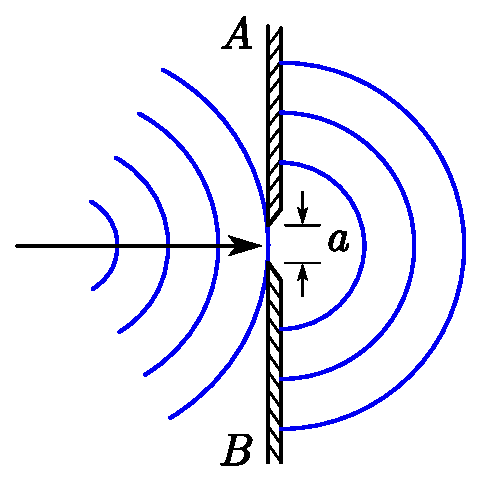
\includegraphics[width=5cm]{./figures/Huygen_1.pdf}
\caption{障碍物的小孔成为新的波源} \label{Huygen_fig1}
\end{figure}

惠更斯(C. Huygens)于1678年提出了关于波传播的几何法则: 在波的传播过程中,波阵面(波前)上的每一点都可行做是发射子波的波源,在其后的任一时刻,这些子波的包迹就成为新的波阵面.这就是\textbf{惠更斯原理(Huygens principle)}.
\begin{figure}[ht]
\centering
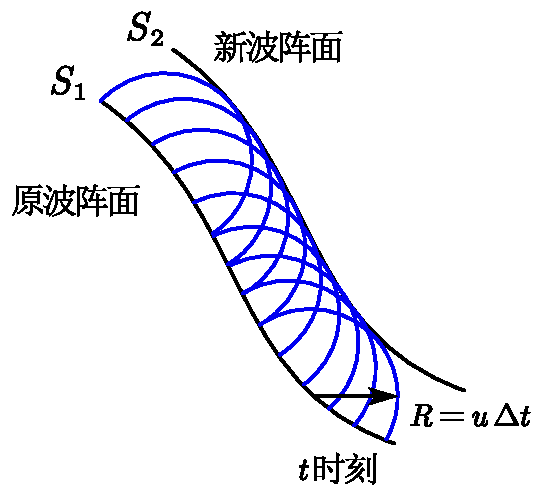
\includegraphics[width=6cm]{./figures/Huygen_2.pdf}
\caption{惠更斯原理} \label{Huygen_fig2}
\end{figure}

如\autoref{Huygen_fig2} 所示,设$S_1$为某一时刻$t $的波阵面,根据惠更斯原理,$S_1$上的每一点发出的球面子波,经$\Delta t$时间后形成半径为$t$的球面,在波的前进方向上,这些子波的包迹$S_2$就成为$t+\Delta t$时刻的新波阵面.惠更斯原理对任何波动过程都是适用的,不论是机械波或电磁波,只要知道某一时刻的波阵面,就可根据这一原理用几何方法来决定任一时刻的波阵面,因而在很广泛的范围内解决了波的传播问题.\autoref{Huygen_fig3} 中用惠更斯原理描绘出球面波和平面波的传播.根据惠更斯原理,还可以简捷地用作图方法说明波在传播中发生的衍射、散射、反射和折射等现象.
\begin{figure}[ht]
\centering
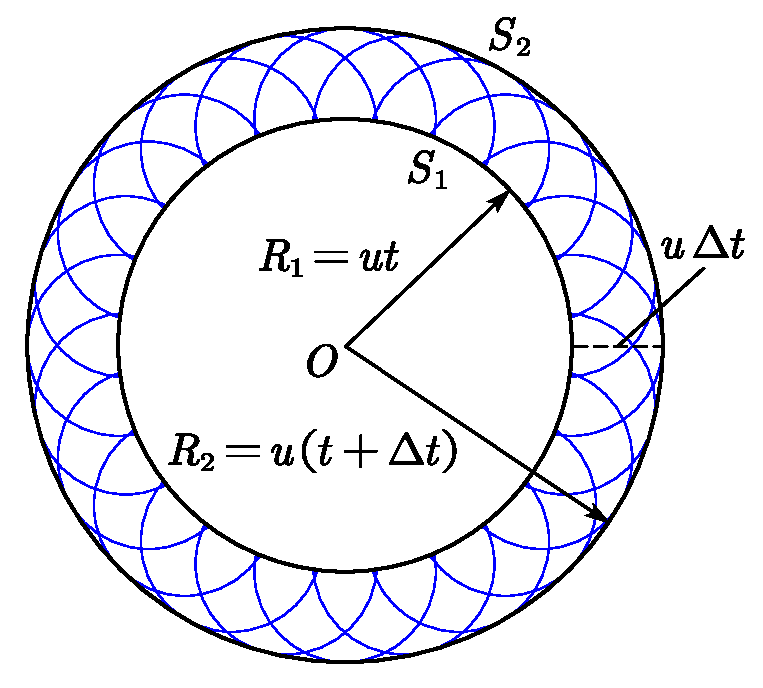
\includegraphics[width=7.5cm]{./figures/Huygen_3.pdf}
\caption{用惠更斯原理求作球面波的新的波阵面} \label{Huygen_fig3}
\end{figure}
\begin{figure}[ht]
\centering
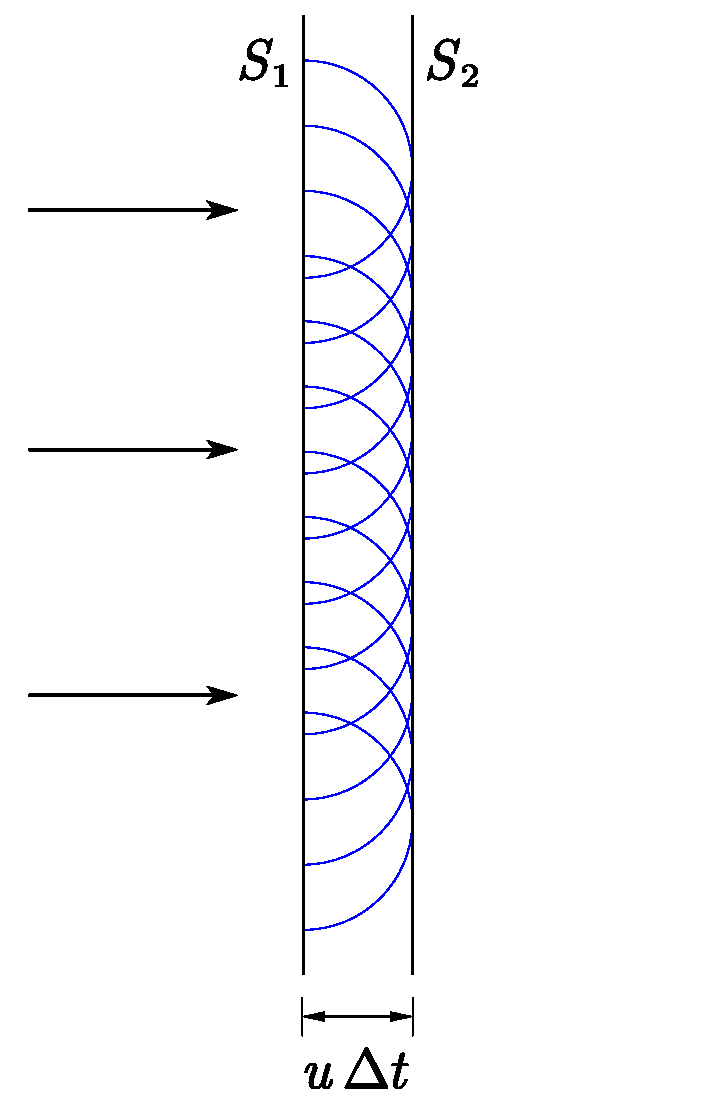
\includegraphics[width=8cm]{./figures/Huygen_4.pdf}
\caption{用惠更斯原理求作平面波的新的波阵面} \label{Huygen_fig4}
\end{figure}
应该指出,惠更斯原理并没有说明各个子波在传播中对某一点振动的相位和振幅究竟有多少贡献,不能给出沿不同方向传播的波的强度分布,后来菲涅耳对惠更斯原理作了补充,这将在惠更斯——菲涅尔原理一节中加以介绍.
